\documentclass[12pt]{article}
\usepackage{amsmath,amssymb,enumerate,enumitem}%la base
\usepackage{fancyhdr}%pour custom les en-têtes et pieds de page
\usepackage{xcolor}%pour les couleurs
\usepackage[a4paper,lmargin=1cm,rmargin=1cm,tmargin=1cm,bmargin=2cm]{geometry}
\usepackage[T1]{fontenc}
\usepackage{hyperref}%hyperliens
\usepackage{graphicx}%images
\usepackage[most]{tcolorbox}%pour les encadrés
\usepackage{import} % pour importer
\usepackage{listings}%pour afficher du code R
\usepackage[pages=some]{background} % pour la page de garde
\usepackage{subcaption}

% --- Couleur violet thème ---
\definecolor{ensae}{RGB}{71, 1, 125}

\hypersetup{
    colorlinks = true,
    linkcolor = ensae!70!white,
    filecolor = ensae,      
    urlcolor = ensae,
    pdfpagemode = FullScreen,
    pdftitle = Linear Time Series Assignment,
    pdfauthor = Alban Géron
}

\pagestyle{fancy}
\lhead{} \rhead{} \lfoot{} \rfoot{}
\renewcommand{\headrulewidth}{0pt}\renewcommand{\footrulewidth}{0pt}

% --- Configuration R ---
\definecolor{codegreen}{rgb}{0,0.6,0}
\definecolor{codegray}{rgb}{0.5,0.5,0.5}
\definecolor{customyellow}{rgb}{1,1,0}
\lstset{
    language=R,                         % R par défaut
    commentstyle=\color{codegreen},
    keywordstyle=\color{blue},
    numberstyle=\tiny\color{codegray},
    stringstyle=\color{magenta},
    basicstyle=\ttfamily,
    breakatwhitespace=false,         
    breaklines=true,                 
    captionpos=b,                    
    keepspaces=true,                 
    numbers=left,                    
    numbersep=3pt,                  
    showspaces=false,                
    showstringspaces=false,
    showtabs=false,                  
    tabsize=2,
    literate=%
        {é}{{\'e}}1 {è}{{\`e}}1 {à}{{\`a}}1 {ù}{{\`u}}1 {â}{{\^a}}1 {ê}{{\^e}}1 {î}{{\^i}}1 {ô}{{\^o}}1 {û}{{\^u}}1
        {É}{{\'E}}1 {È}{{\`E}}1 {À}{{\`A}}1 {Ù}{{\`U}}1 {Â}{{\^A}}1 {Ê}{{\^E}}1 {Î}{{\^I}}1 {Ô}{{\^O}}1 {Û}{{\^U}}1
        {ç}{{\c{c}}}1 {Ç}{{\c{C}}}1
}
\newcommand\rcode[1]{{\lstinline[language=R]!#1!}}

% --- Titres ---
\usepackage{titlesec}
\renewcommand{\thesection}{\Roman{section}} % Titres sections en chiffres romains
\titleformat{\section}{\normalfont\sffamily\bfseries\Large}{\thesection}{1em}{}
\titleformat{\subsection}{\normalfont\sffamily\bfseries\large}{\thesubsection}{1em}{}
\titleformat{\subsubsection}{\normalfont\sffamily\bfseries}{\thesubsubsection}{1em}{}
\setlist[enumerate]{
    font = \color{ensae!70!white}\sffamily,
    leftmargin = *,
    resume
}



\begin{document}
    \backgroundsetup{
        scale = 1,
        angle = 0,
        opacity = 1,
        contents = {
            
\includegraphics[width = \paperwidth, height = \paperheight, keepaspectratio]{bgcover.pdf}
        }
    }
   \BgThispage
    \newgeometry{
        lmargin=1cm,
        rmargin=7cm,
        tmargin=4cm,
        bmargin=4cm
    }
    \thispagestyle{empty} % pas de numérotation pour cette page
    \begin{center}
        
\includegraphics[width=0.8\textwidth]{ensae IP paris.png}

        \vskip4cm

        \Large\bfseries
        \begin{tcolorbox}[
            enhanced, sharp corners,
            colback = ensae!5!white,
            colframe = ensae!60!white,
            boxrule = 0.5pt,
            drop fuzzy shadow = gray
        ]
            \centering {\huge\sffamily ARIMA modelling of a time series}

            \vskip0.3cm

            \emph{\Large Linear Time Series Assignment}
        \end{tcolorbox}

        \vskip4cm

        Alban \textsc{Géron} and Théo \textsc{Lartigau}

        \vskip0.5cm

        Academic year: 2024-2025
    \end{center}

    \newpage
    \restoregeometry

    \section{The data}

    \begin{enumerate}
        \item The chosen series is the \emph{seasonally and working-day adjusted Industrial Production Index (IPI) for the manufacture of beverages}\footnote{\url{https://www.insee.fr/fr/statistiques/serie/010767669}}. It tracks the monthly physical output of France’s drinks industry (breweries, wineries, distillers, soft‑drink plants and bottled‑water facilities), adjusted for calendar and seasonal fluctuations. The index is expressed on a base‑$100$ scale with 2021 as the reference year, that is, a value of $110$ means the beverage industry produced $10 \%$ more than its 2021 average in that month.

        To isolate the monthly industrial production data, rows should be filtered to retain only those whose first column matches the \texttt{YYYY-MM} format. The second column, containing the index values, should then be extracted and converted to numeric form. Because the data appears in reverse chronological order, the values should be reversed to restore proper temporal sequencing.

        Although the base‑$100$ scaling tends to keep the variance relatively stable, a logarithmic transformation may still be considered if volatility appears to increase with the level of the index.

        \item As a first step we have checked the stationarity of the initial series, which we will label $(Y_t)$ in the following. Table \ref{tab:stationarity_tests} summarizes the results of the Augmented Dickey-Fuller (ADF), Phillips-Perron (PP) and Kwiatkowski-Phillips-Schmidt-Shin (KPSS) tests.
        %
        \begin{table}[ht]
            \centering
            \begin{tabular}{l|ccc}
                \textbf{Test} & \textbf{Test Statistic} & \textbf{p-value} & \textbf{Decision} \\
                \hline
                ADF  & -4.7236 & < 0.01 & Stationary \\
                PP   & -148.75 & < 0.01 & Stationary \\
                KPSS & 5.8263  & < 0.01 & Not Stationary
            \end{tabular}
            \caption{Stationarity test results on $(Y_t)$}
            \label{tab:stationarity_tests}
        \end{table}
        
        The results of the three stationarity tests on the initial series are somewhat contradictory. Both the ADF and PP tests reject the null hypothesis of a unit root at the $1 \%$ level, suggesting that the series is stationary. However, the KPSS test rejects the null hypothesis of level stationarity, indicating that the series is not stationary. This discrepancy calls into question the stationarity of $(Y_t)$. To determine the integration order of $(Y_t)$, we test the stationarity of the first-order differenced series $(\nabla Y_t)$. Plotting the series $(\nabla Y_t)$ shows that it seems stationary, see Figure \ref{fig:plot_series_diff}. We then applied the same tests to the first-differenced series to determine its integration order, the results of which can be found in Table \ref{tab:stationarity_tests_diff}.
        %
        \begin{table}[ht]
            \centering
            \begin{tabular}{l|ccc}
                \textbf{Test} & \textbf{Test Statistic} & \textbf{p-value} & \textbf{Decision} \\
                \hline
                ADF  & -10.088  & < 0.01 & Stationary \\
                PP   & -438.51  & < 0.01 & Stationary \\
                KPSS & 0.0465   & > 0.1  & Stationary
            \end{tabular}
            \caption{Stationarity test results on $(\nabla Y_t)$}
            \label{tab:stationarity_tests_diff}
        \end{table}

        Once again, ADF and PP tests reject the null hypothesis of a unit root, however now KPSS accepts the null hypothesis of stationarity. We conclude that $Y_t \sim I(1)$.

        \item Text
        %
        \begin{figure}[h]
            \centering
            \begin{subfigure}[b]{0.49\linewidth}
                \centering
                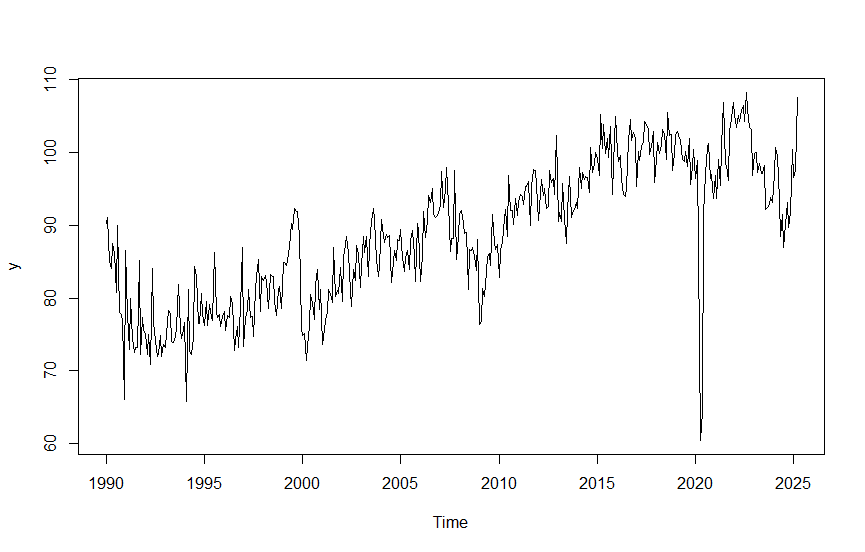
\includegraphics[width=\linewidth]{plot series.png}
                \caption{Initial series}
                \label{fig:plot_series}
            \end{subfigure}
            \hfill
            \begin{subfigure}[b]{0.49\linewidth}
                \centering
                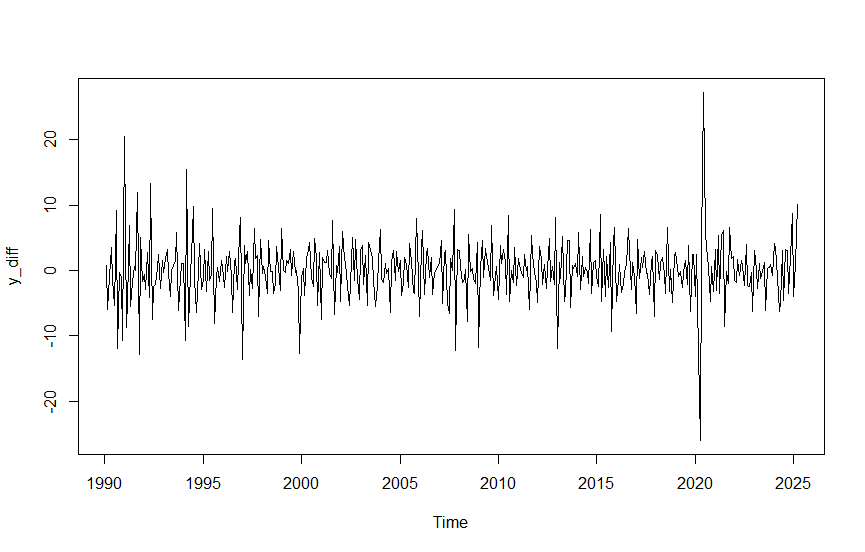
\includegraphics[width=\linewidth]{plot y_diff.png}
                \caption{First-order differenced series}
                \label{fig:plot_series_diff}
            \end{subfigure}
        \end{figure}
    \end{enumerate}

    \section{ARMA models}

    \begin{enumerate}
        \item 
    \end{enumerate}

    % \section{Prediction}
\end{document}